
\section{Raster Maps}
\label{sec-1}
\label{cha:raster}

A raster data structure is a matrix of cells organized into rows and
columns where each cell contains a value representing information,
such as temperature, altitude, population density, land use, etc.
This section describes how to display a raster with two different
examples: CM-SAF solar irradiation rasters will illustrate the use of
quantitative data, and land cover and population data from the
NEO-NASA project will exemplify the display of categorical data and
multivariate rasters. Read Chapter \ref{cha:dataSpatial} for
details about these datasets.

\subsection{Quantitative Data}
\label{sec-1-1}
As an example of quantitative data, this section displays the
distribution of annual solar irradiation over the Iberian peninsula
using the estimates from CM SAF. The \texttt{RasterLayer} object of annual
averages of solar irradiation estimated by CM SAF can be easily
displayed with the \texttt{levelplot} method of the \texttt{rasterVis}
package. Figure \ref{fig:levelplotCMSAF} illustrates this raster with
marginal graphics to show the column (longitude) and row (latitude)
summaries of the \texttt{RasterLayer} object. The summary is computed with
the function defined by \texttt{FUN.margin} (which uses \texttt{mean} as the default
value).

\index{Packages!raster@\texttt{raster}}
\index{Packages!rasterVis@\texttt{rasterVis}}
\index{levelplot@\texttt{levelplot}}
\index{rasterTheme@\texttt{rasterTheme}}

\lstset{language=R,numbers=none}
\begin{lstlisting}
library(raster)
library(rasterVis)
SISav <- raster('data/SISav')
levelplot(SISav)
\end{lstlisting}

\begin{figure}[htb]
\centering
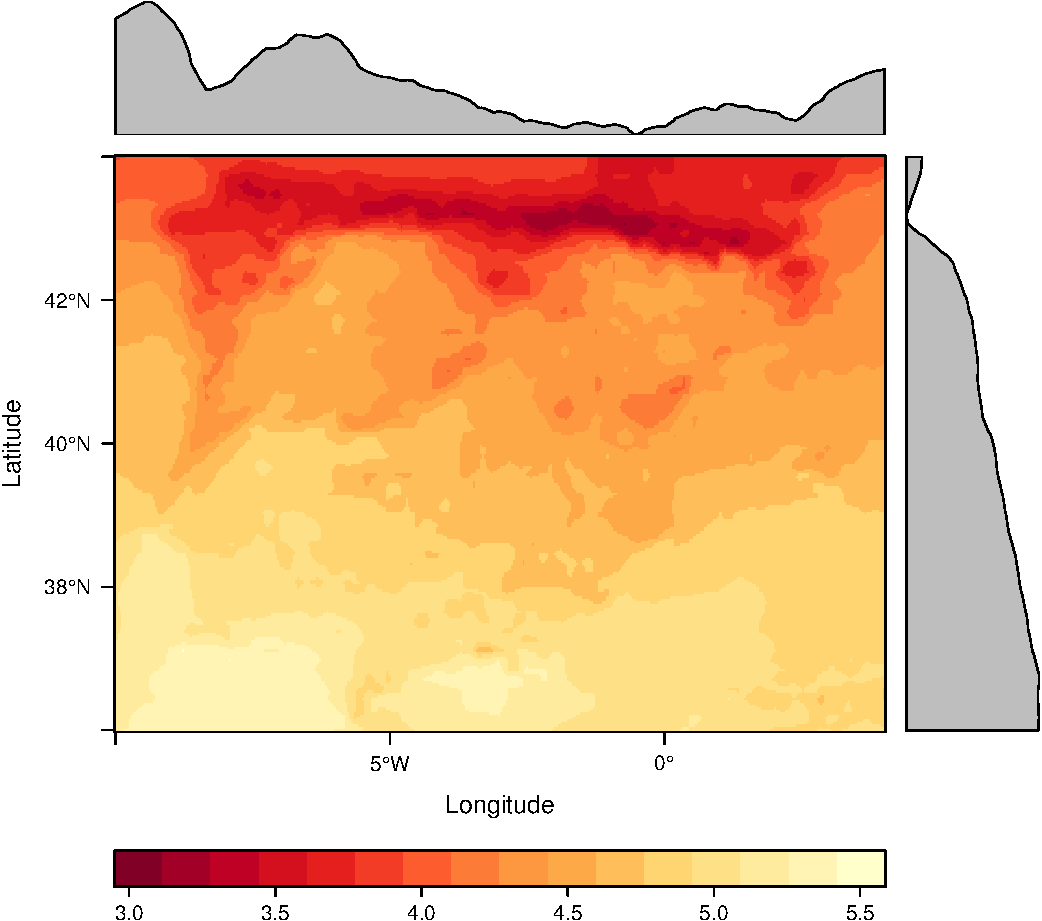
\includegraphics[width=.9\linewidth]{figs/leveplotSISavOrig.pdf}
\caption{\label{fig:levelplotCMSAF}Annual average of solar radiation displayed with a sequential palette.}
\end{figure}

Although the solar irradiation distribution reveals the physical
structure of the region, it is recommended to add the geographic
context with a layer of administrative boundaries (Figure
\ref{fig:levelplotCMSAF_boundaries}).

\index{Packages!maps@\texttt{maps}}
\index{Packages!mapdata@\texttt{mapdata}}
\index{Packages!maptools@\texttt{maptools}}
\index{map2SpatialLines@\texttt{map2SpatialLines}}

\lstset{language=R,numbers=none}
\begin{lstlisting}
library(maps)
library(mapdata)
library(maptools)

ext <- as.vector(extent(SISav))
boundaries <- map('worldHires',
		  xlim=ext[1:2], ylim=ext[3:4],
		  plot=FALSE)
boundaries <- map2SpatialLines(boundaries,
			       proj4string=CRS(projection(SISav)))
\end{lstlisting}

\index{Packages!sp@\texttt{sp}}
\index{Packages!latticeExtra@\texttt{latticeExtra}}
\index{sp.lines@\texttt{sp.lines}}

\lstset{language=R,numbers=none}
\begin{lstlisting}
levelplot(SISav) + layer(sp.lines(boundaries, lwd=0.5))
\end{lstlisting}

\begin{figure}[htb]
\centering
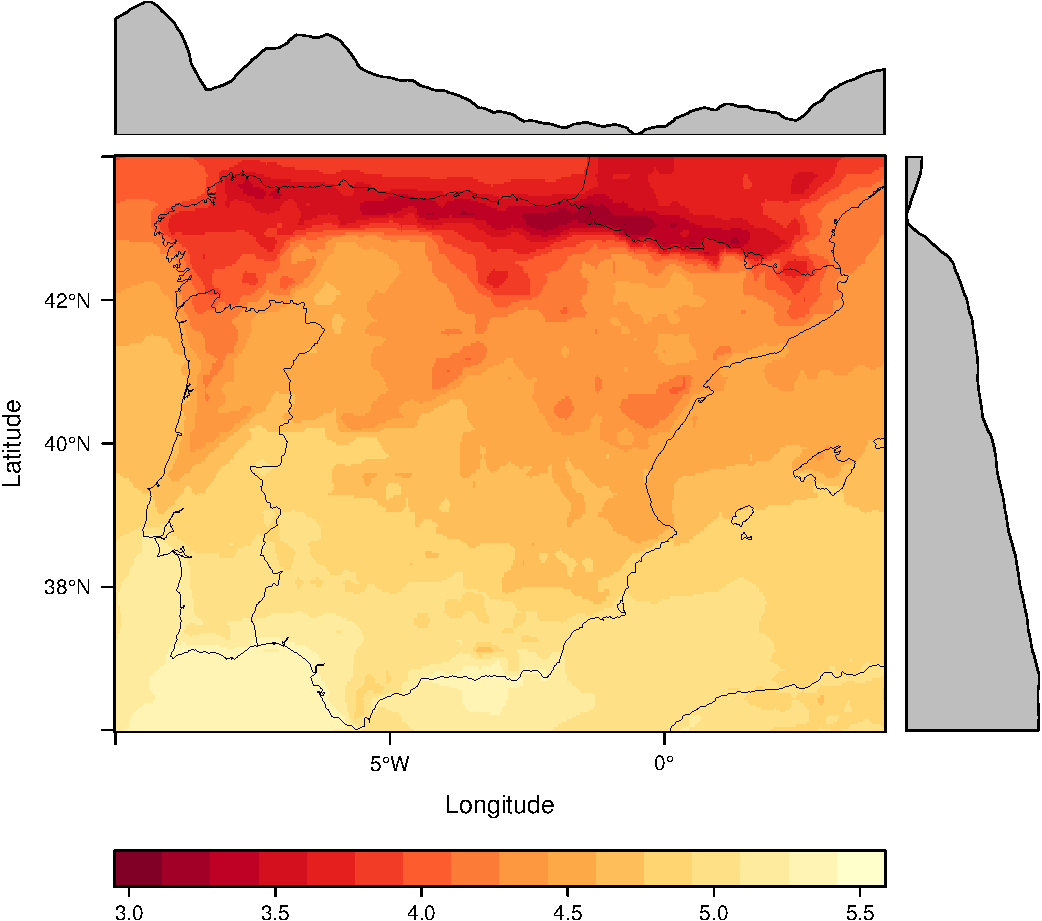
\includegraphics[width=.9\linewidth]{figs/leveplotSISavBoundaries.pdf}
\caption{\label{fig:levelplotCMSAF_boundaries}Annual average of solar radiation with administrative boundaries.}
\end{figure}

\subsubsection{Hill Shading}
\label{sec-1-1-1}
A frequent method to improve the display of meteorological rasters is
the hill shading or shaded relief technique, a method of representing
relief on a map by depicting the shadows that would be cast by high
ground if light comes from a certain sun position (Figure
\ref{fig:hillShading}).

The procedure is as follows:

\begin{itemize}
\item Download a Digital Elevation Model (DEM) from the DIVA-GIS service.
\end{itemize}
\index{Data!DIVA-GIS}

\lstset{language=R,numbers=none}
\begin{lstlisting}
old <- setwd(tempdir())
download.file('http://www.diva-gis.org/data/msk_alt/ESP_msk_alt.zip', 'ESP_msk_alt.zip')
unzip('ESP_msk_alt.zip', exdir='.')

DEM <- raster('ESP_msk_alt')
\end{lstlisting}

\begin{itemize}
\item Compute the hill shade raster with \texttt{terrain} and \texttt{hillShade} from \texttt{raster}.
\end{itemize}
\index{terrain@\texttt{terrain}}
\index{hillShade@\texttt{hillShade}}

\lstset{language=R,numbers=none}
\begin{lstlisting}
slope <- terrain(DEM, 'slope')
aspect <- terrain(DEM, 'aspect')
hs <- hillShade(slope=slope, aspect=aspect,
		angle=20, direction=30)
\end{lstlisting}
\lstset{language=R,numbers=none}
\begin{lstlisting}
setwd(old)
\end{lstlisting}

\begin{itemize}
\item Combine the result with the previous map using semitransparency.
\end{itemize}
\index{+.trellis@\texttt{+.trellis}}
\index{layer@\texttt{layer}}

\lstset{language=R,numbers=none}
\begin{lstlisting}
## hillShade theme: gray colors and semitransparency
hsTheme <- modifyList(GrTheme(), list(regions=list(alpha=0.6)))

levelplot(SISav, panel=panel.levelplot.raster,
	  margin=FALSE, colorkey=FALSE) +
    levelplot(hs, par.settings=hsTheme, maxpixels=1e6) +
    layer(sp.lines(boundaries, lwd=0.5))
\end{lstlisting}

\begin{figure}[htb]
\centering
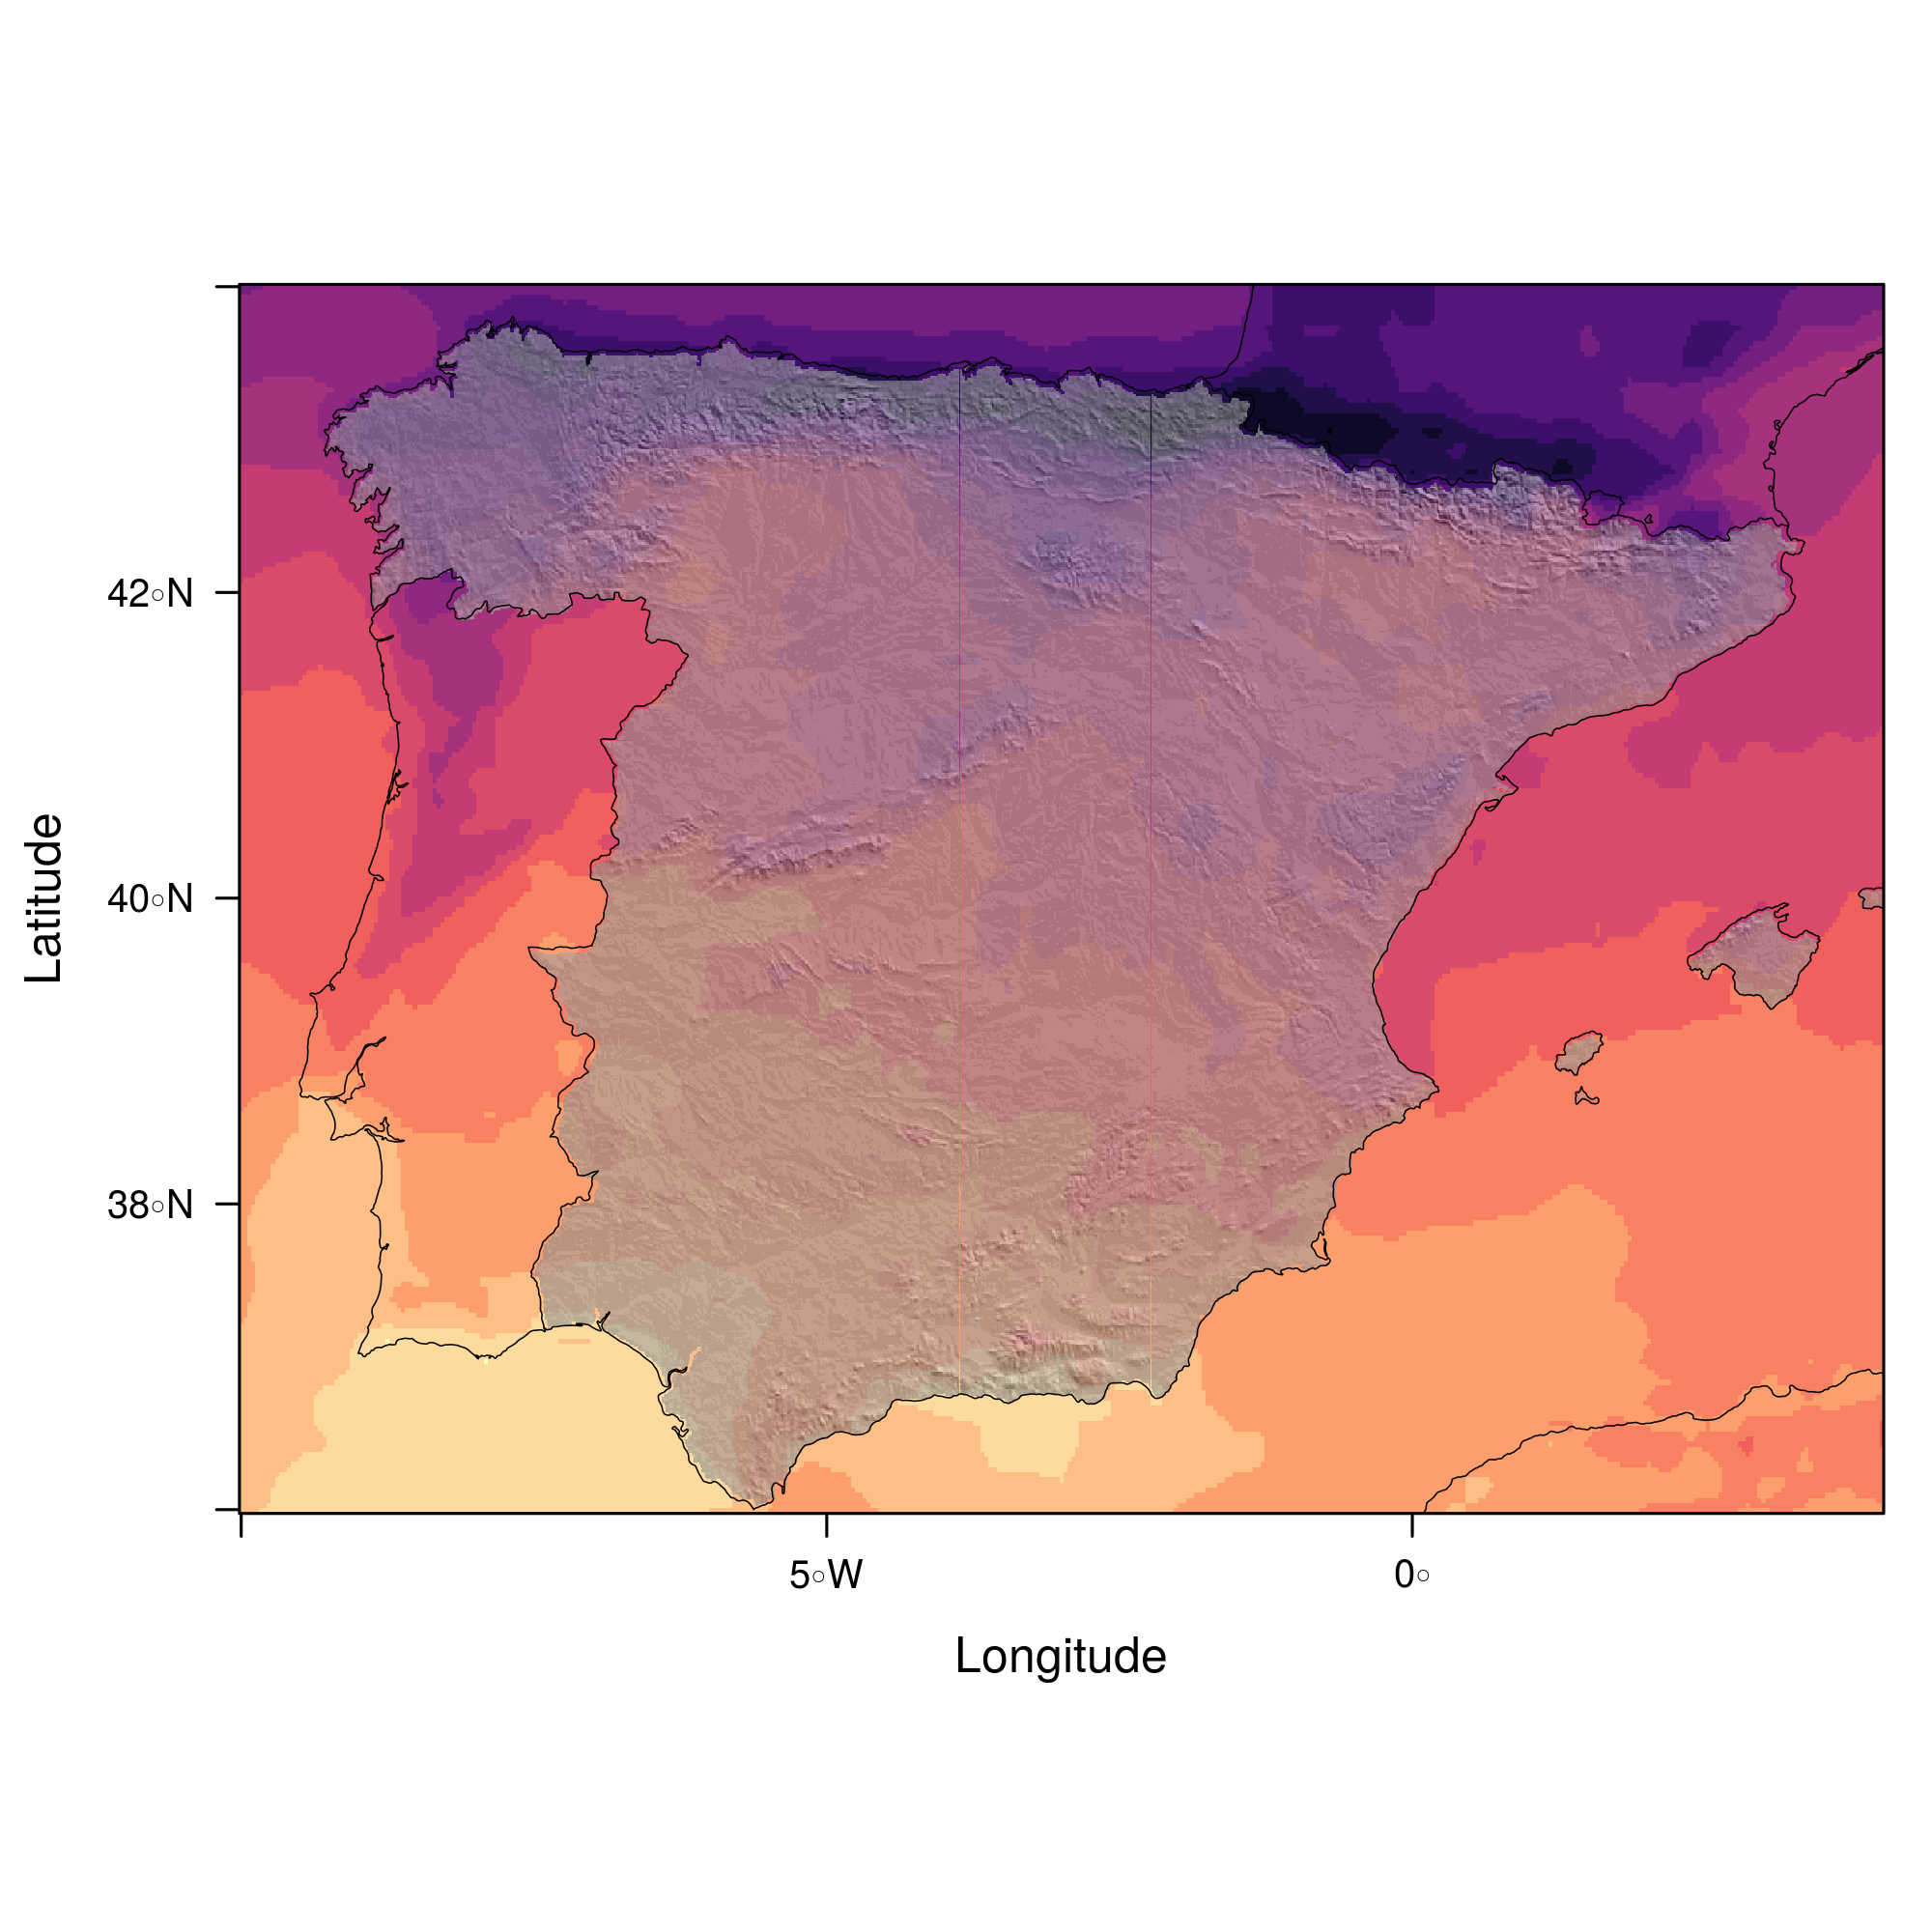
\includegraphics[width=.9\linewidth]{figs/hillShading.png}
\caption{\label{fig:hillShading}Hill shading of annual average of solar radiation.}
\end{figure}
\subsubsection{Excursus: 3D Visualization}
\label{sec-1-1-2}
An alternative method for a DEM is 3D visualization where the user can
rotate or zoom the figure. This solution is available thanks to the
\texttt{rgl} package, which provides functions for 3D interactive
graphics. The \texttt{plot3D} function in the \texttt{rasterVis} package is a
wrapper to this package for \texttt{RasterLayer} objects.

\index{Packages!rgl@\texttt{rgl}}
\index{3D visualization}
\index{WebGL}
\index{STL}

\lstset{language=R,numbers=none}
\begin{lstlisting}
plot3D(DEM, maxpixels=5e4)
\end{lstlisting}

The output scene can be exported to several formats such as WebGL with
\texttt{writeWebGL} to be rendered in a browser, or \texttt{STL} with \texttt{writeSTL}, a
format commonly used in 3D printing. Files using this format are
viewed easily on GitHub (Figure \ref{fig:DEM_STL})

\lstset{language=R,numbers=none}
\begin{lstlisting}
writeSTL('figs/DEM.stl')
\end{lstlisting}

\begin{figure}
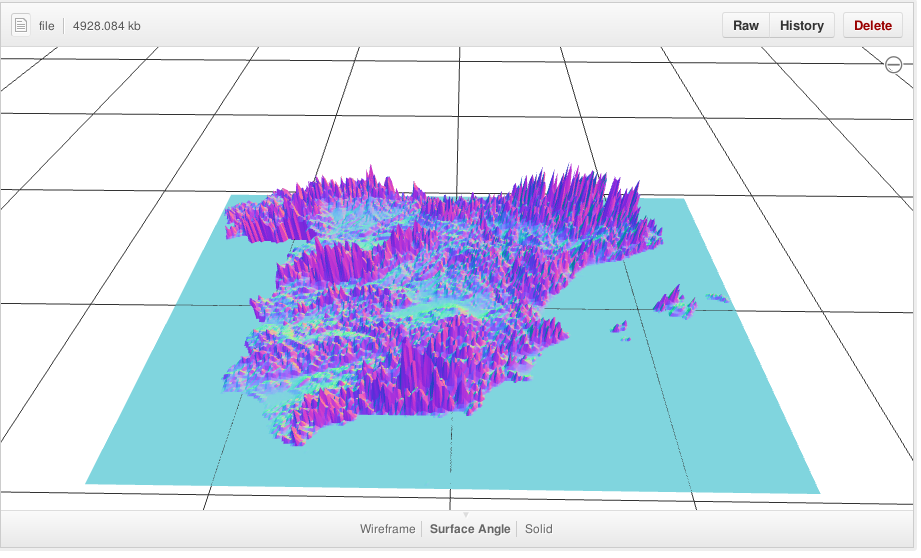
\includegraphics[height=0.3\textheight]{figs/DEM_STL_GitHub.png}
\caption{\label{fig:DEM_STL}3D visualization of a Digital Elevation
  Model using the STL format in a GitHub repository.}
\end{figure}

\subsubsection{Diverging Palettes}
\label{sec-1-1-3}
Next, instead of displaying the absolute values of each cell, we will
analyze the differences between each cell and the global average
value. This average is computed with the \texttt{cellStats} function and
substracted from the original \texttt{RasterLayer}. Figure
\ref{fig:xyplotSISav} displays the relation between these scaled
values and latitude (\texttt{y}), with five different groups defined by the
longitude (\texttt{cut(x, 5)}). It is evident that larger irradiation values
are associated with lower latitudes. However, there is no such clear
relation between irradiation and longitude.

\index{cellStats@\texttt{cellStats}}

\lstset{language=R,numbers=none}
\begin{lstlisting}
meanRad <- cellStats(SISav, 'mean')
SISav <- SISav - meanRad
\end{lstlisting}

\index{xyplot@\texttt{xyplot}}
\index{rasterTheme@\texttt{rasterTheme}}
\index{Packages!hexbin@\texttt{hexbin}}
\index{plinrain@\texttt{plinrain}}

\lstset{language=R,numbers=none}
\begin{lstlisting}
xyplot(layer ~ y, data = SISav,
       groups=cut(x, 5),
       par.settings=rasterTheme(symbol=plinrain(n=5, end=200)),
       xlab = 'Latitude', ylab = 'Solar radiation (scaled)',  
       auto.key=list(space='right', title='Longitude', cex.title=1.3))
\end{lstlisting}

\begin{figure}[htb]
\centering
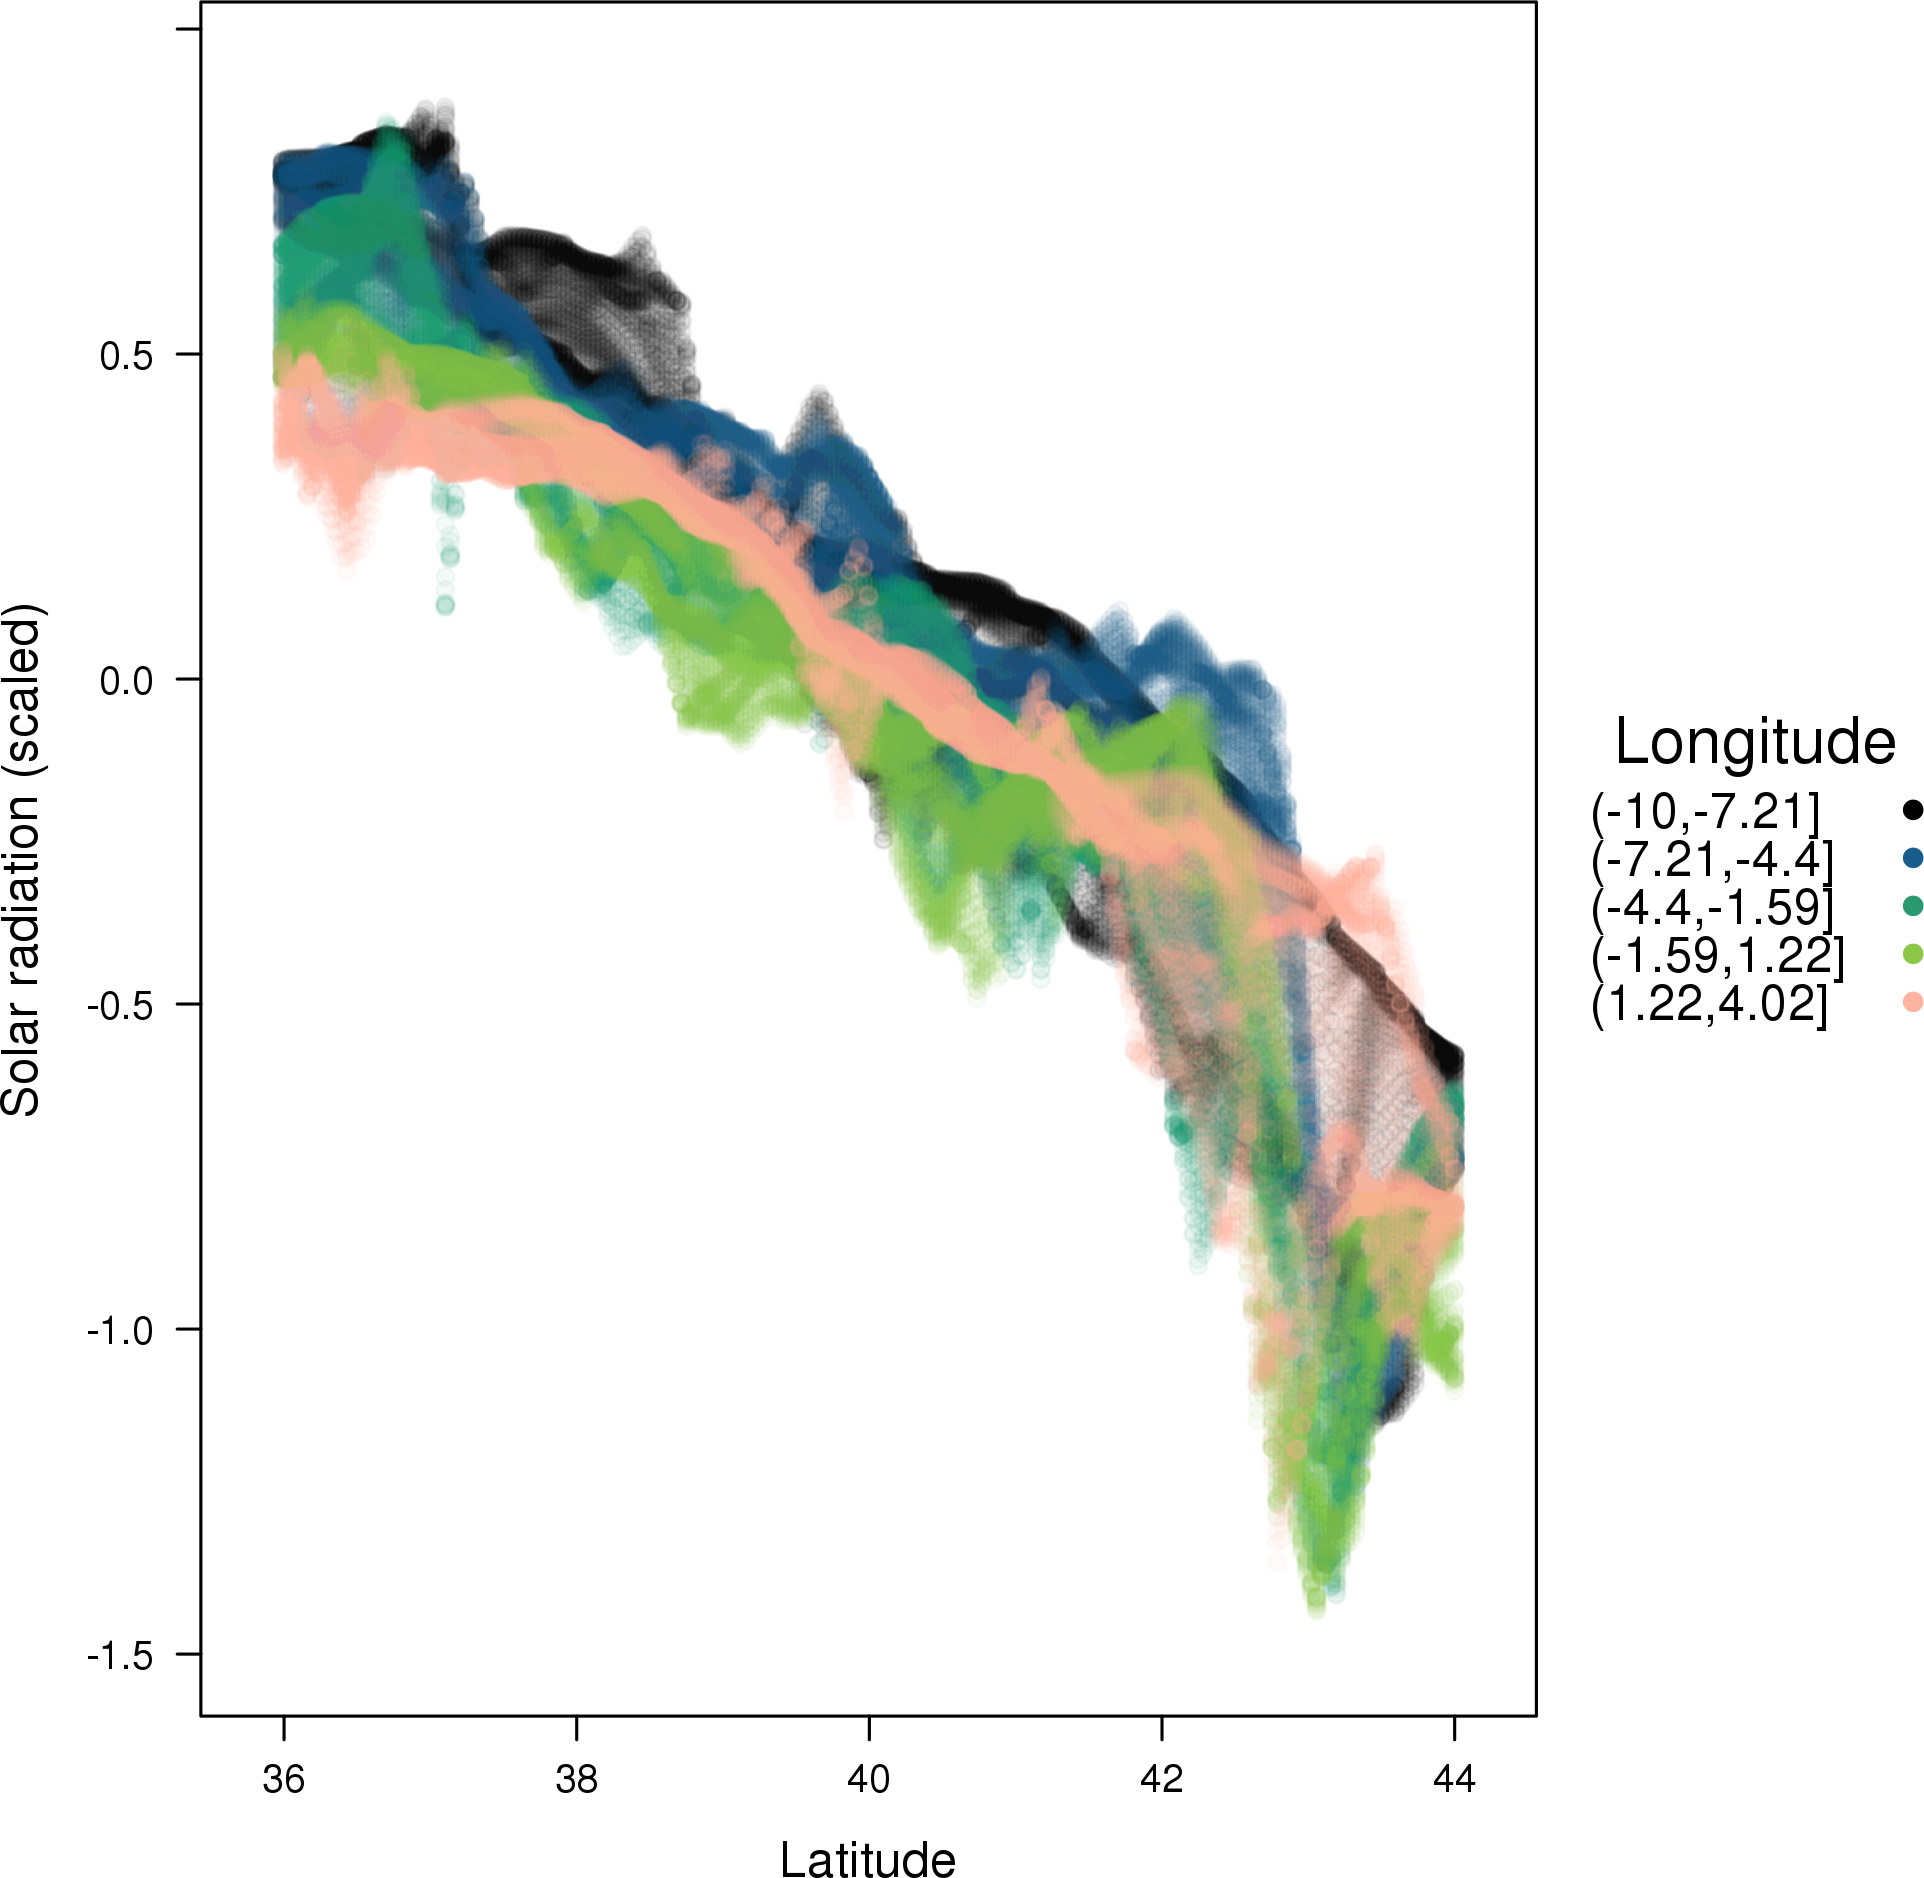
\includegraphics[width=.9\linewidth]{figs/xyplotSISav.png}
\caption{\label{fig:xyplotSISav}Relation between scaled annual average radiation and latitude for several longitude groups.}
\end{figure}

Numerical information ranging in an interval including a neutral
value is commonly displayed with diverging palettes. These
palettes represent neutral classes with light colors, while low
and high extremes of the data range are highlighted using dark
colors with contrasting hues. I use the Purple-Orange palette from
ColorBrewer with purple for positive values and orange for
negative values. In order to underline the position of the
interval containing zero, the center color of this palette is
substituted with pure white. The resulting palette is displayed in
Figure \ref{fig:showDivPal} with the custom \texttt{showPal}
function. The corresponding correspondent raster map produced with this palette
is displayed in Figure \ref{fig:divPal_SISav_naive}.  Although
extreme positive and negative values can be easily discriminated,
the zero value is not associated with white because the data range
is not symmetrical around zero.

\index{Package!RColorBrewer@\texttt{RColorBrewer}}
\index{brewer.pal@\texttt{brewer.pal}}

\lstset{language=R,numbers=none}
\begin{lstlisting}
divPal <- brewer.pal(n=9, 'PuOr')
divPal[5] <- "#FFFFFF"

showPal <- function(pal, labs=pal, cex=0.6, ...){
  barplot(rep(1, length(pal)), col=pal,
	  names.arg=labs, cex.names=cex,
	  axes=FALSE, ...)
}

showPal(divPal)
\end{lstlisting}

\begin{figure}[htb]
\centering
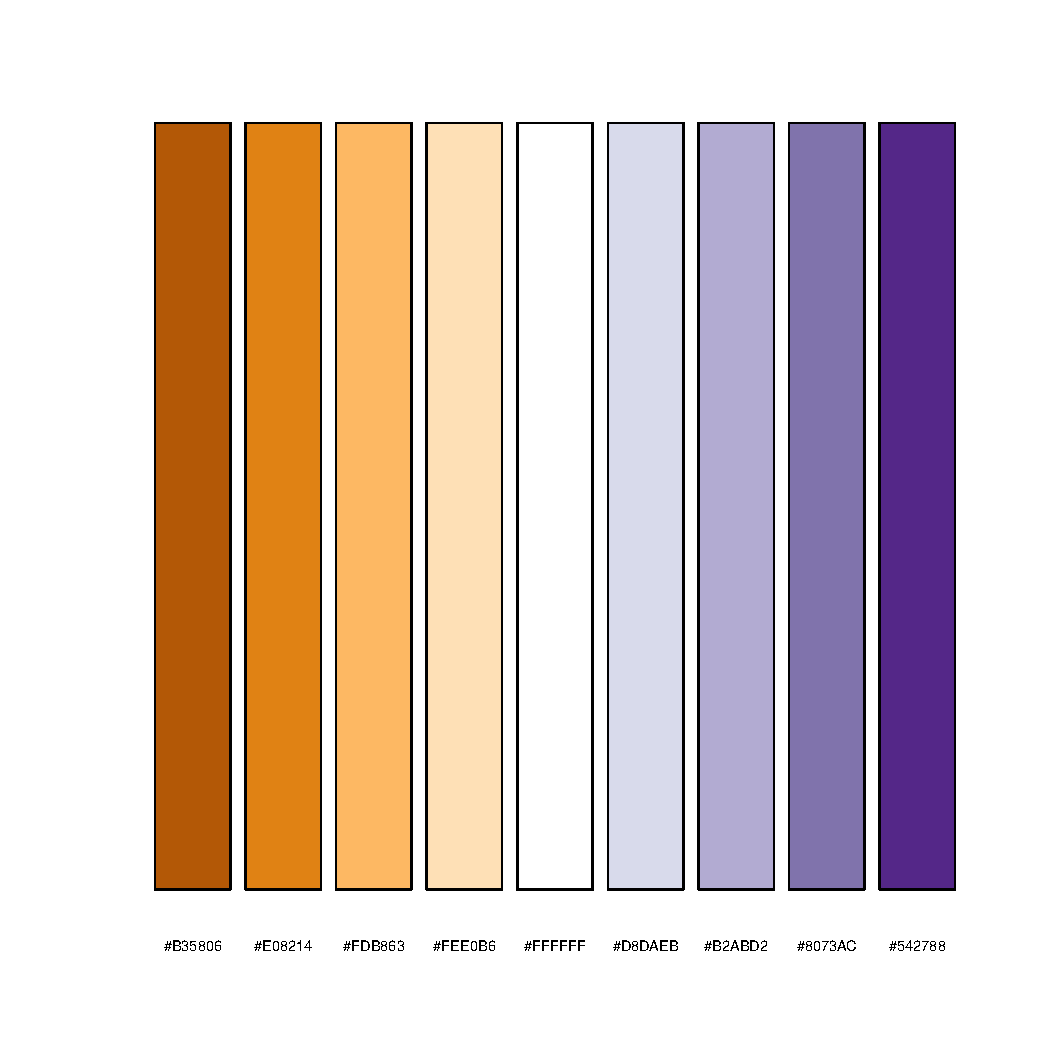
\includegraphics[height=0.3\textheight]{figs/showDivPal.pdf}
\caption{\label{fig:showDivPal}Purple-Orange diverging palette using white as middle color.}
\end{figure}


\lstset{language=R,numbers=none}
\begin{lstlisting}
divTheme <- rasterTheme(region=divPal)

levelplot(SISav, contour=TRUE, par.settings=divTheme)
\end{lstlisting}

\begin{figure}[htb]
\centering
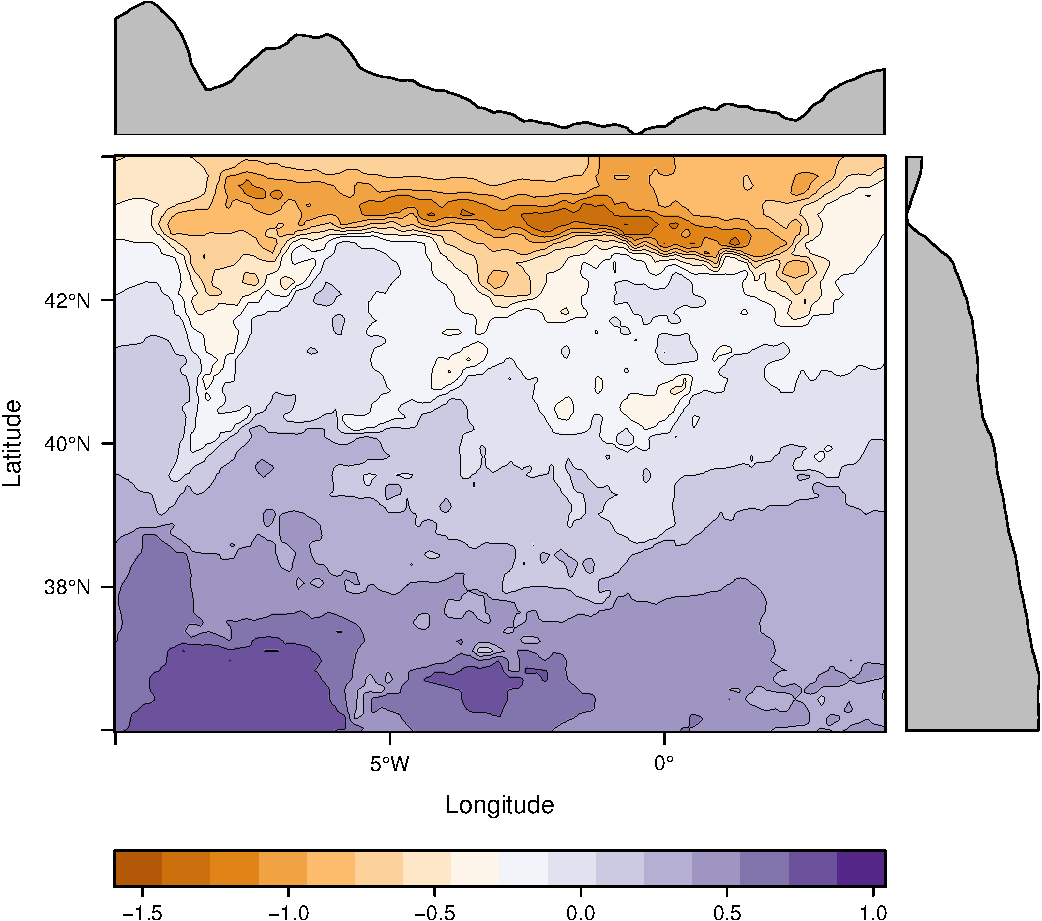
\includegraphics[width=.9\linewidth]{figs/divPal_SISav_naive.pdf}
\caption{\label{fig:divPal_SISav_naive}Asymmetric raster data (scaled annual average irradiation) displayed with a symmetric diverging palette.}
\end{figure}

The solution is to connect the symmetrical color palette with the
asymmetrical data range. The first step is to create a set of
breaks such that the zero value is the center of one of the
intervals.
\lstset{language=R,numbers=none}
\begin{lstlisting}
rng <- range(SISav[])
## Number of desired intervals
nInt <- 15
## Increment corresponding to the range and nInt
inc0 <- diff(rng)/nInt
## Number of intervals from the negative extreme to zero
n0 <- floor(abs(rng[1])/inc0)
## Update the increment adding 1/2 to position zero in the center of an interval
inc <- abs(rng[1])/(n0 + 1/2)
## Number of intervals from zero to the positive extreme
n1 <- ceiling((rng[2]/inc - 1/2) + 1)
## Collection of breaks
breaks <- seq(rng[1], by=inc, length= n0 + 1 + n1)
\end{lstlisting}

The next step is to compute the midpoints of each interval. These
points represent the data belonging to each interval, and their value
will be connected with a color of the palette.
\index{findInterval@\texttt{findInterval}}
\index{tapply@\texttt{tapply}}

\lstset{language=R,numbers=none}
\begin{lstlisting}
## Midpoints computed with the median of each interval
idx <- findInterval(SISav[], breaks, rightmost.closed=TRUE)
mids <- tapply(SISav[], idx, median)
## Maximum of the absolute value both limits
mx <- max(abs(breaks))
mids
\end{lstlisting}

A simple method to relate the palette and the intervals is with a
straight line such that a point is defined by the absolute maximum
value, (\texttt{(mx, 1)}), and another point by zero, (\texttt{(0, 0.5)}).  Why are
we using the interval [0, 1] as the \texttt{y}-coordinate of this line, and
why is 0.5 the result of zero? The reason is that the input of the
\texttt{break2pal} function will be the result of \texttt{colorRamp}, a function
that creates another interpolating function which maps colors with
values between 0 and 1. Therefore, a new palette is created,
extracting colors from the original palette, such that the central
color (white) is associated with the interval containing zero. This
palette is displayed in Figure \ref{fig:showBreak2Pal}.

The raster map produced with this new palette is displayed in Figure
\ref{fig:divPalSISav}. Now zero is clearly associated with the white
color.
\index{colorRamp@\texttt{colorRamp}}
\index{rgb@\texttt{rgb}}
\lstset{language=R,numbers=none}
\begin{lstlisting}
break2pal <- function(x, mx, pal){
  ## x = mx gives y = 1
  ## x = 0 gives y = 0.5
  y <- 1/2*(x/mx + 1)
  rgb(pal(y), maxColorValue=255)
}

## Interpolating function that maps colors with [0, 1]
## rgb(divRamp(0.5), maxColorValue=255) gives "#FFFFFF" (white)
divRamp <- colorRamp(divPal)
## Diverging palette where white is associated with the interval
## containing the zero
pal <- break2pal(mids, mx, divRamp)
showPal(pal, round(mids, 1))
\end{lstlisting}

\begin{figure}[htb]
\centering
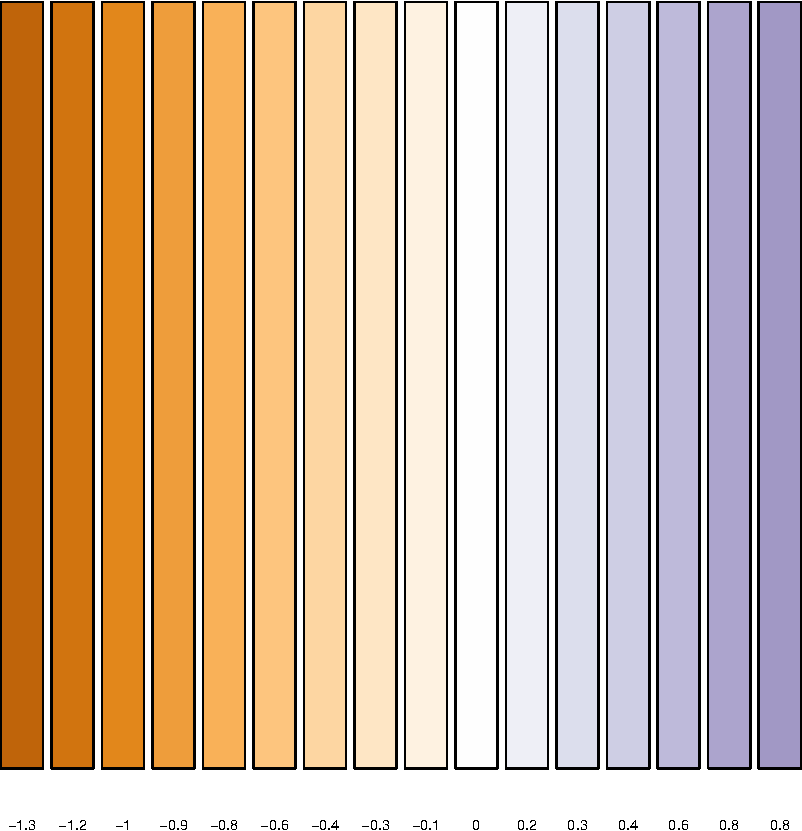
\includegraphics[height=0.3\textheight]{figs/showBreak2Pal.pdf}
\caption{\label{fig:showBreak2Pal}Modified diverging palette related with the asymmetrical raster data.}
\end{figure}


\lstset{language=R,numbers=none}
\begin{lstlisting}
levelplot(SISav, par.settings=rasterTheme(region=pal),
	  at=breaks, contour=TRUE)
\end{lstlisting}

\begin{figure}[htb]
\centering
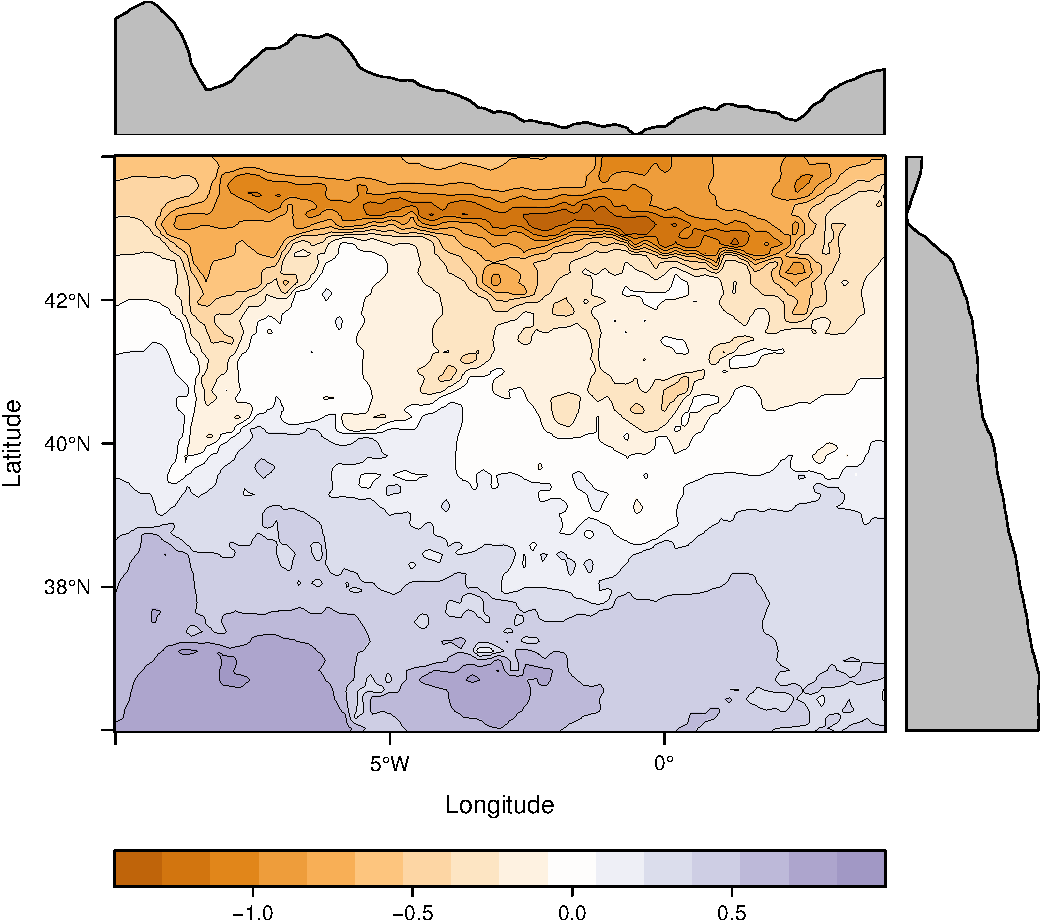
\includegraphics[width=.9\linewidth]{figs/divPalSISav.pdf}
\caption{\label{fig:divPalSISav}Asymmetric raster data (scaled annual average irradiation) displayed with a modified diverging palette.}
\end{figure}


It is interesting to note two operations carried out internally by
the \texttt{lattice} package. First, the \texttt{custom.theme} function (used by
\texttt{rasterTheme}) creates a new palette with 100 colors using
\texttt{colorRampPalette} to interpolate the palette passed as an
argument. Second, the \texttt{level.colors} function makes the
arrangement between intervals and colors. If this function
receives more colors than intervals, it chooses a subset of the
palette disregarding some of the intermediate colors. Therefore,
because this function will receive 100 colors from \texttt{par.settings}, it
is difficult to control exactly which colors of our original
palette will be represented.

An alternative way for finer control is to fill the \texttt{regions\$col}
component of the theme with our palette after it has been created
(Figure \ref{fig:divPal_SISav_regions}).

\lstset{language=R,numbers=none}
\begin{lstlisting}
divTheme <- rasterTheme()

divTheme$regions$col <- pal
levelplot(SISav, par.settings=divTheme, at=breaks, contour=TRUE)
\end{lstlisting}

\begin{figure}[htb]
\centering
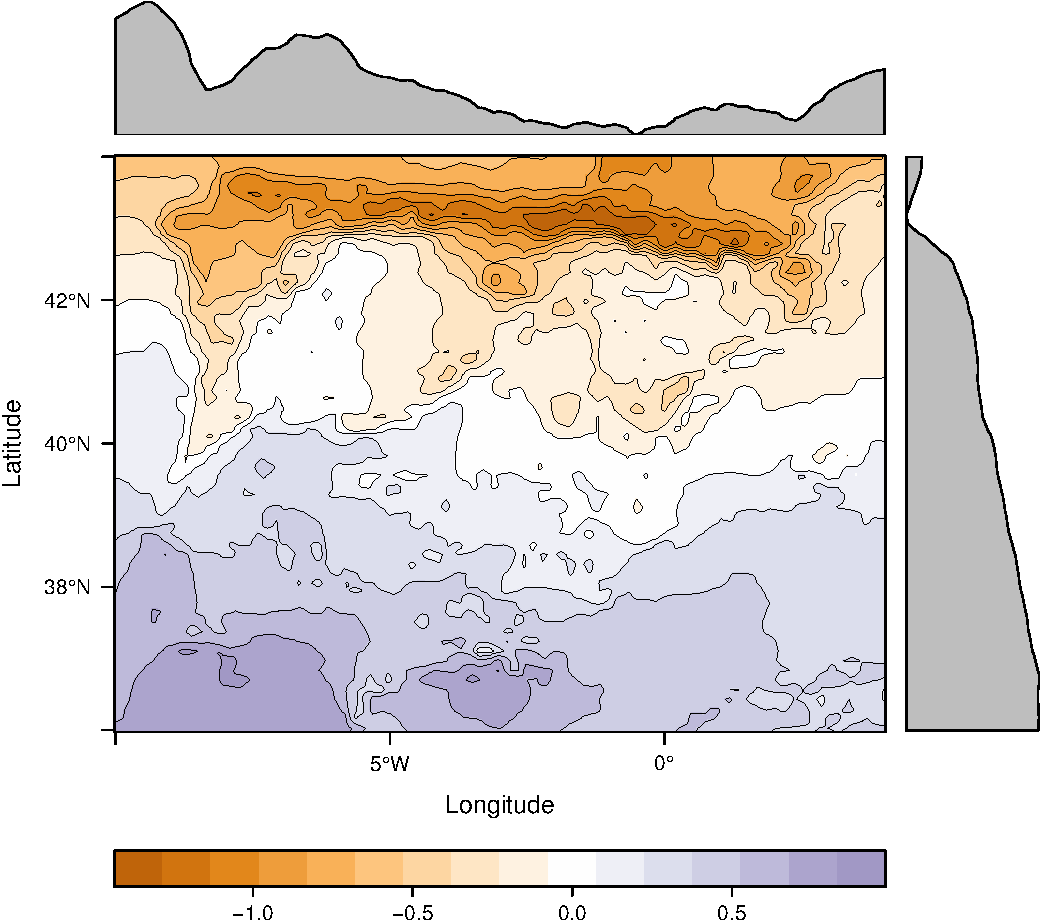
\includegraphics[width=.9\linewidth]{figs/divPalSISav_regions.pdf}
\caption{\label{fig:divPal_SISav_regions}Same as Figure \ref{fig:divPalSISav} but colors are assigned directly to the \texttt{regions\$col} component of the theme.}
\end{figure}

A final improvement to this map is to compute the intervals using a
classification algorithm with the \texttt{classInt} package. With this
approach it is likely that zero will not be perfectly centered in its
corresponding interval. The remaining code is exactly the same as
above, replacing the \texttt{breaks} vector with the result of the
\texttt{classIntervals} function. Figure \ref{fig:divPalSISav_classInt}
displays the result.

\index{Packages!classInt@\texttt{classInt}}
\index{classIntervals@\texttt{classIntervals}}

\lstset{language=R,numbers=none}
\begin{lstlisting}
library(classInt)

cl <- classIntervals(SISav[],
		     ## n=15, style='equal')
		     ## style='hclust')
		     ## style='sd')
		     style='kmeans')
		     ## style='quantile')
cl
breaks <- cl$brks
\end{lstlisting}

\lstset{language=R,numbers=none}
\begin{lstlisting}
idx <- findInterval(SISav[], breaks, rightmost.closed=TRUE)
mids <- tapply(SISav[], idx, median)
mids
mx <- max(abs(breaks))
pal <- break2pal(mids, mx, divRamp)
divTheme$regions$col <- pal
levelplot(SISav, par.settings=divTheme, at=breaks, contour=TRUE)
\end{lstlisting}

\begin{figure}[htb]
\centering
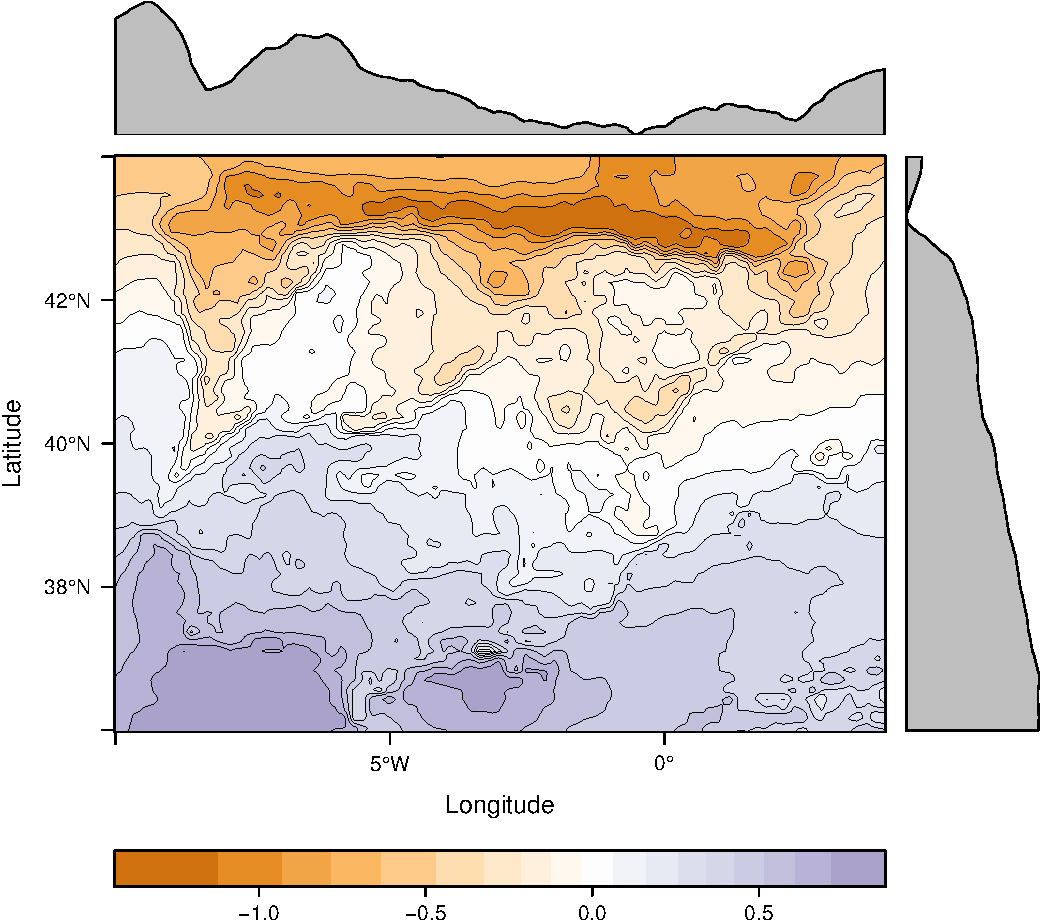
\includegraphics[width=.9\linewidth]{figs/divPalSISav_classInt.pdf}
\caption{\label{fig:divPalSISav_classInt}Same as Figure \ref{fig:divPal_SISav_regions} but defining intervals with the optimal classification method.}
\end{figure}

\subsection{Categorical Data}
\label{sec-1-2}
Land cover is the observed physical cover on the Earth's surface. A
set of seventeen different categories is commonly used. Using
satellite observations, it is possible to map where on Earth each of
these seventeen land surface categories can be found and how these
land covers change over time.

This section illustrates how to read and display rasters with
categorical information using information from the NEO-NASA
project. After the land cover and population density files have been
downloaded, two \texttt{RasterLayers} can be created with the \texttt{raster}
package. Both files are read, their geographical extent reduced to the
area of India and China, and cleaned (\texttt{99999} cells are replaced with
\texttt{NA}).

\index{Packages!raster@\texttt{raster}}
\index{extent@\texttt{extent}}
\index{crop@\texttt{crop}}

\lstset{language=R,numbers=none}
\begin{lstlisting}
library(raster)
## China and India  
ext <- extent(65, 135, 5, 55)

pop <- raster('875430rgb-167772161.0.FLOAT.TIFF')
pop <- crop(pop, ext)
pop[pop==99999] <- NA

landClass <- raster('241243rgb-167772161.0.TIFF')
landClass <- crop(landClass, ext)
\end{lstlisting}

Each land cover type is designated with a different key: the sea is
labeled with 0; forests with 1 to 5; shrublands, grasslands, and
wetlands with 6 to 11; agriculture and urban lands with 12 to 14; and
snow and barren with 15 and 16.  These four groups (sea is replaced by
\texttt{NA}) will be the levels of the categorical raster. The \texttt{raster}
package includes the \texttt{ratify} method to define a layer as categorical
data, filling it with integer values associated to a Raster Attribute
Table (RAT).


\index{ratify@\texttt{ratify}}
\index{cut@\texttt{cut}}

\lstset{language=R,numbers=none}
\begin{lstlisting}
landClass[landClass %in% c(0, 254)] <- NA
## Only four groups are needed:
## Forests: 1:5
## Shrublands, etc: 6:11
## Agricultural/Urban: 12:14
## Snow: 15:16
landClass <- cut(landClass, c(0, 5, 11, 14, 16))
## Add a Raster Attribute Table and define the raster as categorical data
landClass <- ratify(landClass)
## Configure the RAT: first create a RAT data.frame using the
## levels method; second, set the values for each class (to be
## used by levelplot); third, assign this RAT to the raster
## using again levels
rat <- levels(landClass)[[1]]
rat$classes <- c('Forest', 'Land', 'Urban', 'Snow')
levels(landClass) <- rat
\end{lstlisting}

This categorical raster can be displayed with the \texttt{levelplot} method
of the \texttt{rasterVis} package. Previously, a theme is defined with the
background color set to \texttt{lightskyblue1} to display the sea areas
(filled with \texttt{NA} values), and the region palette is defined with
adequate colors (Figure \ref{fig:landClass}).

\index{Packages!rasterVis@\texttt{rasterVis}}
\index{levelplot@\texttt{levelplot}}
\index{modifyList@\texttt{modifyList}}
\index{rasterTheme@\texttt{rasterTheme}}

\lstset{language=R,numbers=none}
\begin{lstlisting}
library(rasterVis)

pal <- c('palegreen4', # Forest
	 'lightgoldenrod', # Land
	 'indianred4', # Urban
	 'snow3')      # Snow

catTheme <- modifyList(rasterTheme(),
		       list(panel.background = list(col='lightskyblue1'),
			    regions = list(col= pal)))

levelplot(landClass, maxpixels=3.5e5, par.settings=catTheme,
	  panel=panel.levelplot.raster)
\end{lstlisting}

\begin{figure}[htb]
\centering
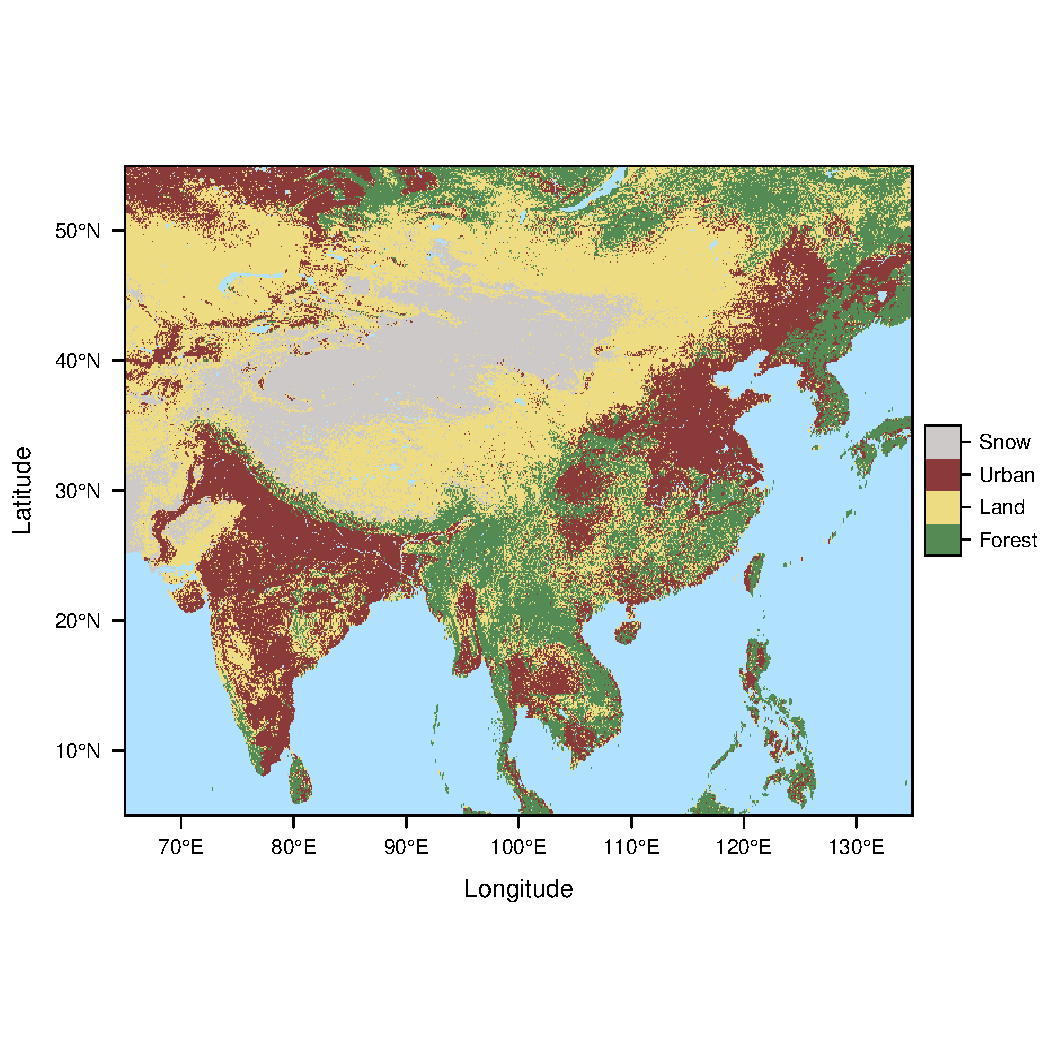
\includegraphics[width=.9\linewidth]{figs/landClass.pdf}
\caption{\label{fig:landClass}Land cover raster (categorical data).}
\end{figure}

Let's explore the relation between the land cover and population
density rasters. Figure \ref{fig:populationNASA} displays this
latter raster using a logarithmic scale.

\lstset{language=R,numbers=none}
\begin{lstlisting}
pPop <- levelplot(pop, zscaleLog=10, par.settings=BTCTheme,
		  maxpixels=3.5e5, panel=panel.levelplot.raster)
pPop
\end{lstlisting}

\begin{figure}[htb]
\centering
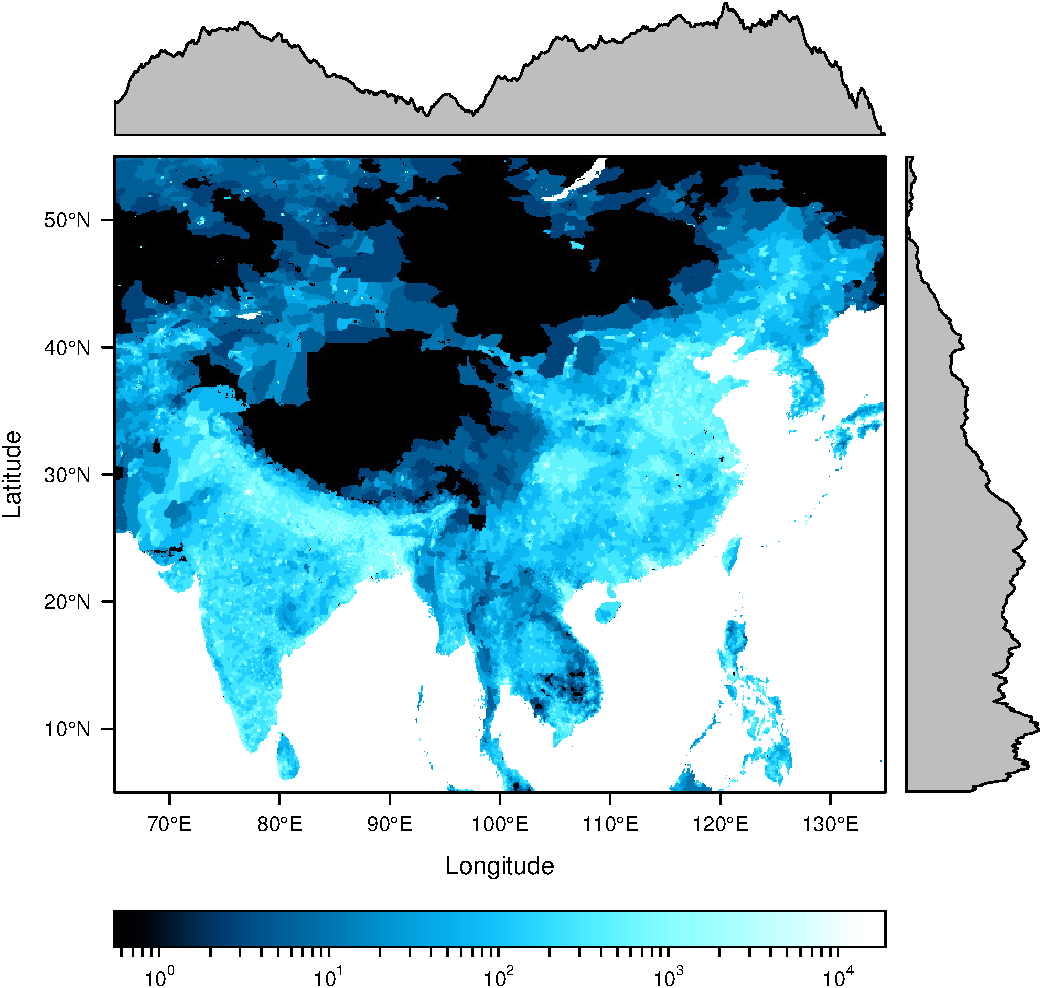
\includegraphics[width=.9\linewidth]{figs/populationNASA.pdf}
\caption{\label{fig:populationNASA}Population density raster.}
\end{figure}

Both rasters can be joined together with the \texttt{stack} method to
create a new \texttt{RasterStack} object. Figure
\ref{fig:histogramLandClass} displays the distribution of the
logarithm of the population density associated to each land class.

\index{stack@\texttt{stack}}
\index{histogram@\texttt{histogram}}

\lstset{language=R,numbers=none}
\begin{lstlisting}
s <- stack(pop, landClass)
names(s) <- c('pop', 'landClass')
histogram(~log10(pop)|landClass, data=s,
	  scales=list(relation='free'))
\end{lstlisting}

\begin{figure}[htb]
\centering
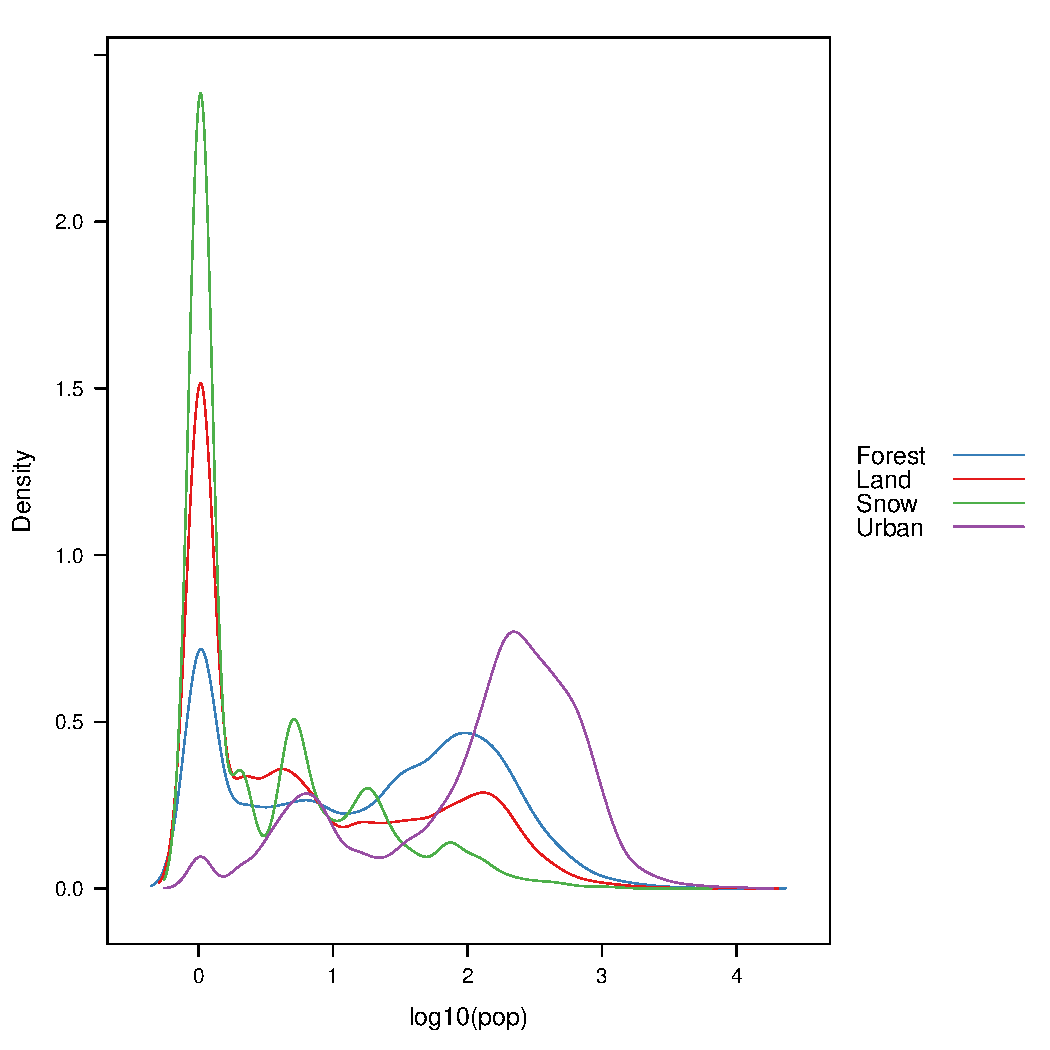
\includegraphics[width=.9\linewidth]{figs/histogramLandClass.pdf}
\caption{\label{fig:histogramLandClass}Distribution of the logarithm of the population density associated to each land class.}
\end{figure}

\subsection{\floweroneleft  Multivariate Legend}
\label{sec-1-3}
We can reproduce the code used to create the multivariate
choropleth (Section \ref{sec:multiChoropleth}) using the
\texttt{levelplot} function from the \texttt{rasterVis} package. Again, the
result is a list of \texttt{trellis} objects. Each of these objects is
the representation of the population density in a particular land
class. The \texttt{+.trellis} function of the \texttt{latticeExtra} package with
\texttt{Reduce} superposes the elements of this list and produces a
\texttt{trellis} object. Figure \ref{fig:popLandClass} displays the
result.




\lstset{language=R,numbers=none}
\begin{lstlisting}
library(colorspace)
## at for each sub-levelplot is obtained from the global levelplot
at <- pPop$legend$bottom$args$key$at
classes <- rat$classes
nClasses <- length(classes)

pList <- lapply(1:nClasses, function(i){
  landSub <- landClass
  ## Those cells from a different land class are set to NA...
  landSub[!(landClass==i)] <- NA
  ## ... and the resulting raster masks the population raster
  popSub <- mask(pop, landSub)
  ## The HCL color wheel is divided in nClasses
  step <- 360/nClasses
  ## and a sequential palette is constructed with a hue from one of
  ## the color wheel parts
  cols <- rev(sequential_hcl(16, h = (30 + step*(i-1))%%360))

  pClass <- levelplot(popSub, zscaleLog=10, at=at,
		      maxpixels=3.5e5,
		      ## labels only needed in the last legend
		      colorkey=(if (i==nClasses) TRUE else list(labels=list(labels=rep('', 17)))),
		      col.regions=cols, margin=FALSE)
})
\end{lstlisting}


\begin{figure}[htb]
\centering
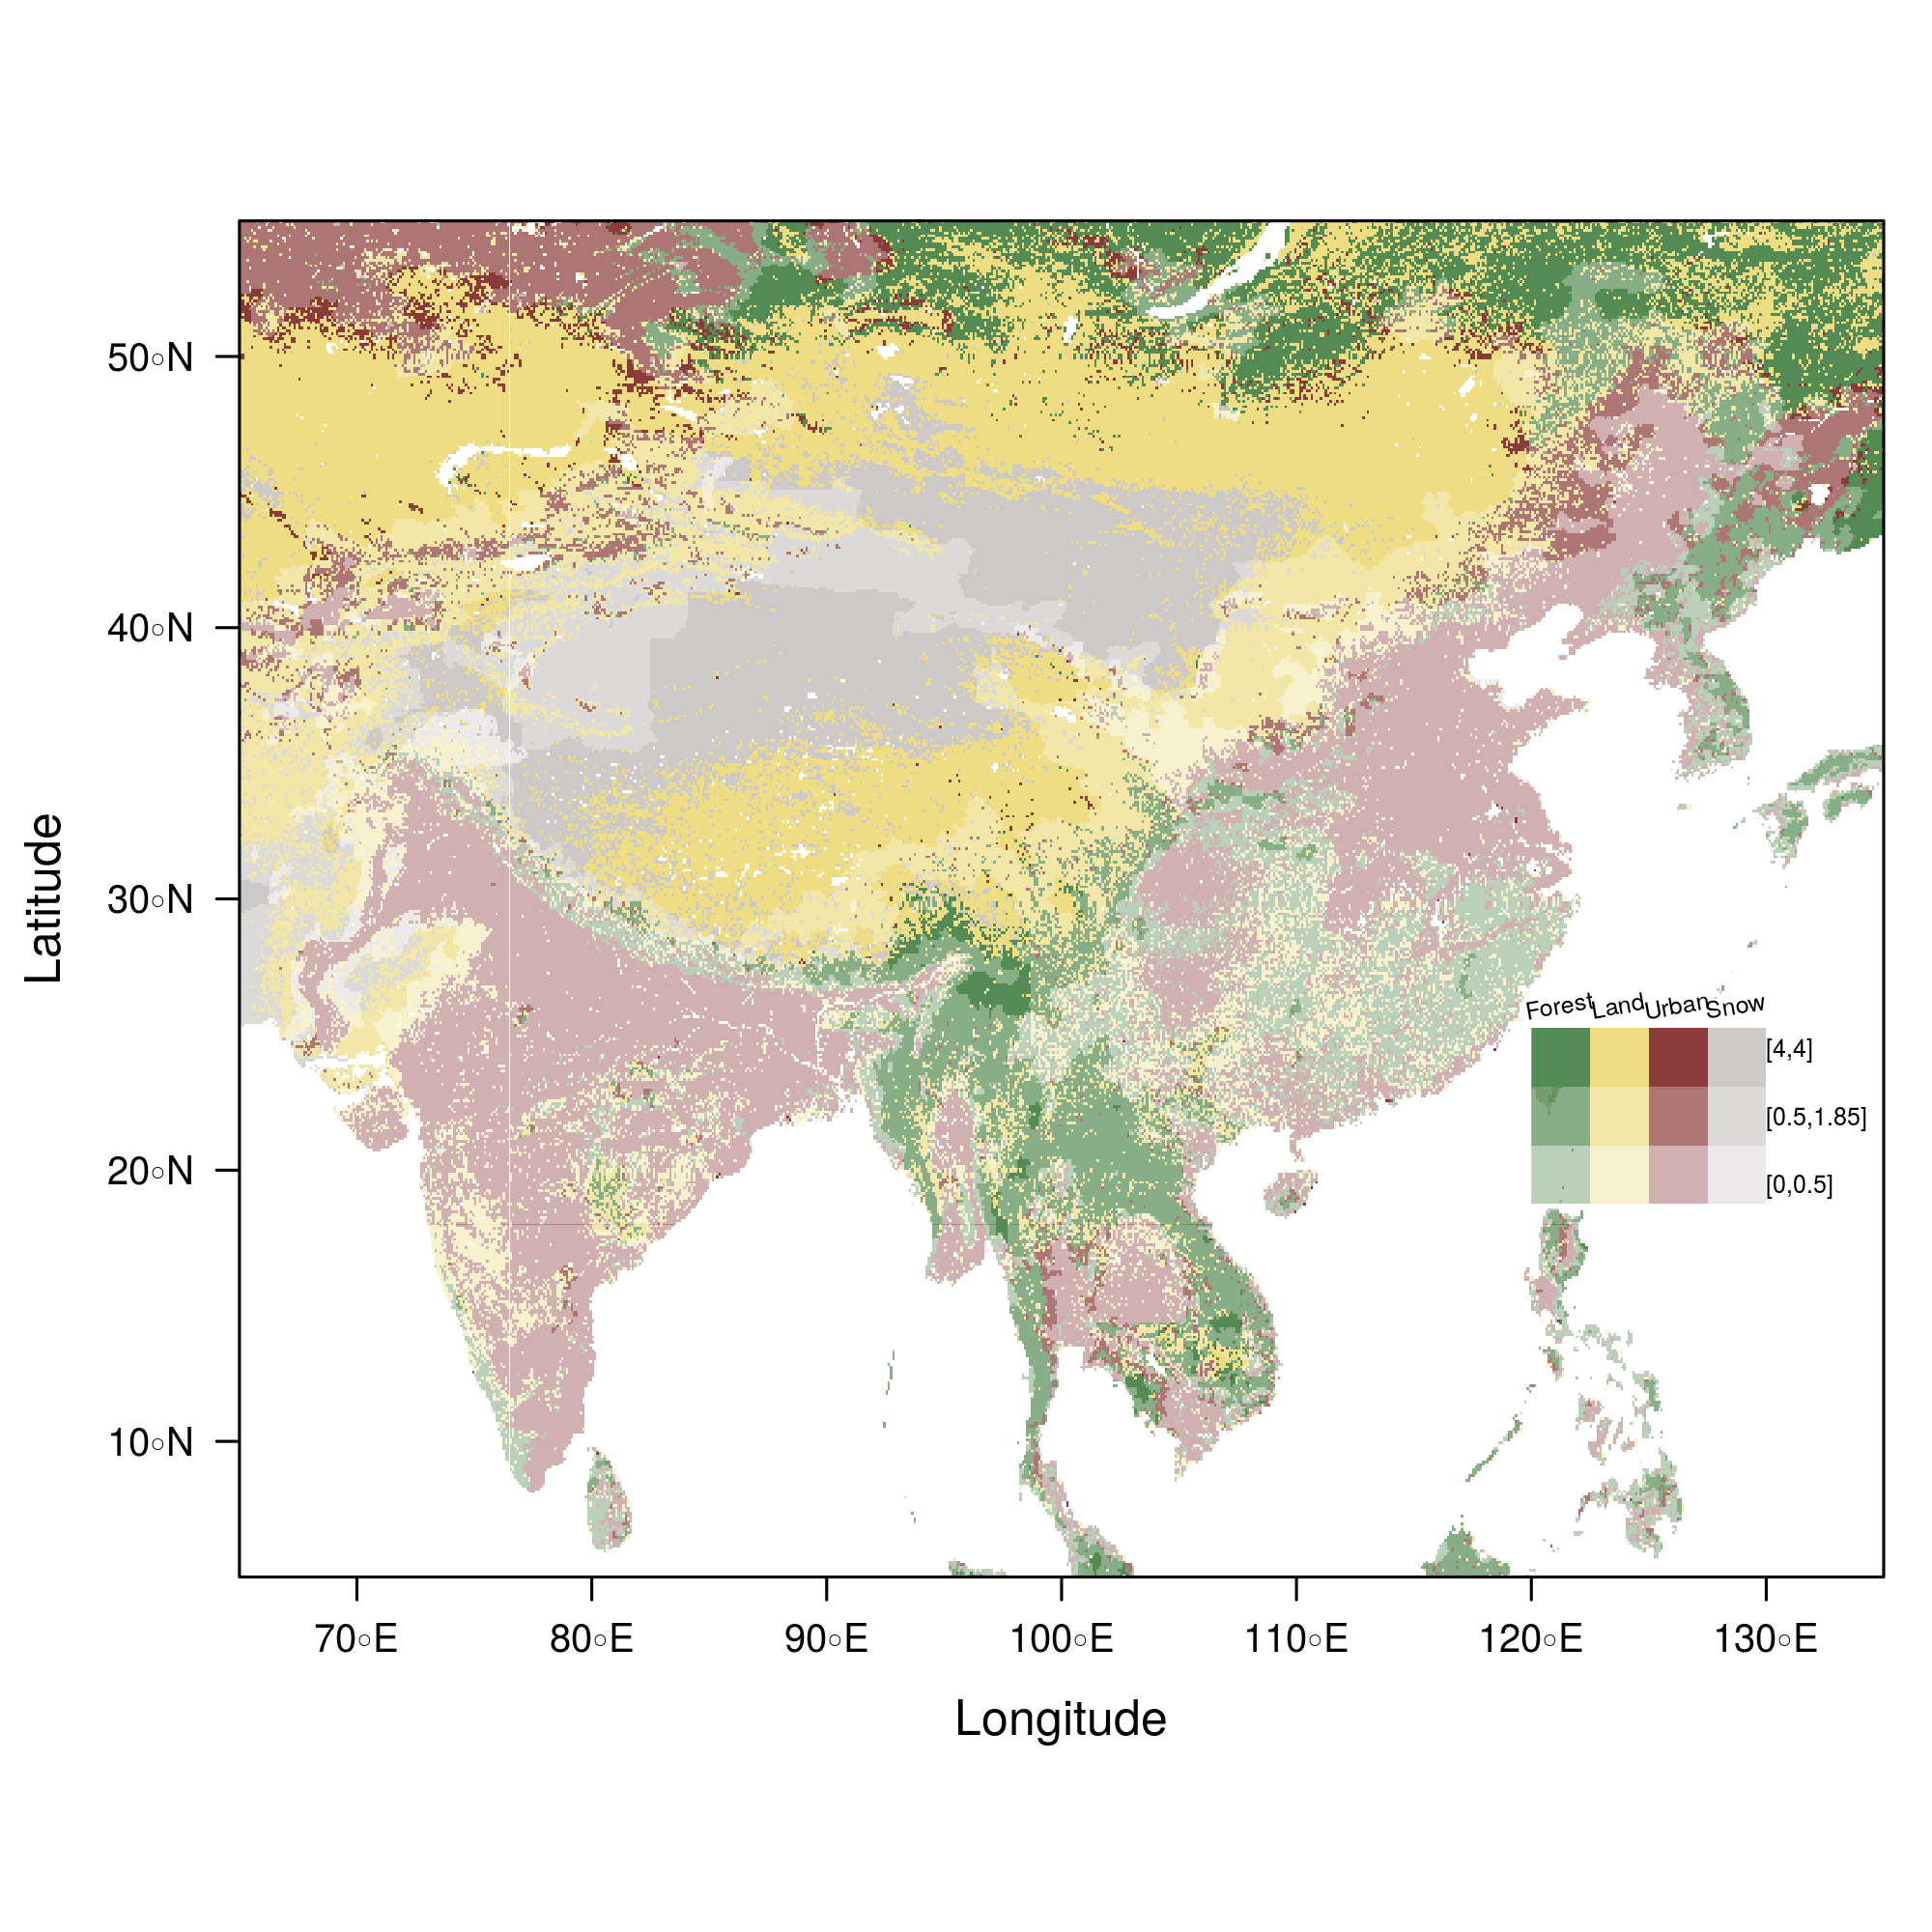
\includegraphics[width=.9\linewidth]{figs/popLandClass.png}
\caption{\label{fig:popLandClass}Population density for each land class (multivariate raster).}
\end{figure}
